\documentclass[a4paper]{article}
\usepackage[sorting=none]{biblatex}
\addbibresource{safe-devicelocatorui.bib}
\usepackage[T1]{fontenc}
\usepackage[utf8]{inputenc}
\usepackage[italian]{babel}
\usepackage{csquotes}
\usepackage{enumitem}
\usepackage{menukeys}
\begin{document}


\makeatletter

\newcommand\setnewpathsep[1]
{%
    \tw@declare@style@simple*{paths}{%
       {\ttfamily\CurrentMenuElement}%
    }[%
       #1%
    ]{blacknwhite}
}

\author{Lorenzo Tanganelli \and Luca Patarca \and Nico Trionfetti}
\title{Safe-Device Locator UI}
\maketitle

\newpage
\tableofcontents

\newpage

\addcontentsline{toc}{section}{Introduzione}
\section*{{Introduzione}}
Il progetto di ricerca industriale \citetitle{SAFE}\cite{SAFE} ha come obbiettivo la realizzazione di sistemi di arredo innovativi capaci di trasformarsi in sistemi inteligenti di protezione passiva delle persone in caso di crollo dell'edificio causato da un terremoto.

Questi sistemi di arredo smart saranno dotati di sensoristica "salva-vita" capace di pre-allertare in caso di terremoto, di rilevare e localizzare la presenza di vita dopo un crollo, di monitorare le condizioni ambientali sotto le macerie e di elaborare e trasmettere informazioni utili a chi deve portare soccorso.

Il ciclo di vita dei sensori si divide in tre scenari operativi:
\begin{enumerate}[label=\roman{*}., ref=(\roman{*})]
    \item \textbf{Tempo di pace:} monitoraggio per il pre-allertamento (es. misure accellerometriche)
    \item \textbf{Durante l'evento:} invio dei dati per il rilevamento dei danni (es. misure accellerometriche, inclinometriche e di spostamento) e attivazione di logiche di intervento in seguito al riconoscimento dell'evento.
    \item \textbf{Dopo l'evento:} invio dei dati per la localizzazione delle vittime e monitoraggio ambientale al fine di guidare gli operatori nel triage di soccorso.
    \end{enumerate}

L'invio di dati tra i sensori ed il mondo esterno avviene utilizzando la tecnologia LoRa.\newline
LoRa consente trasmissioni a lungo raggio e a basso consumo energetico arrivando oltre 10 km nelle zone rurali e 3–5 km in zone fortemente urbanizzate.\cite{s18030772}

Facendo riferimento al modello ISO/OSI la tecnologia è presente in due strati: 
\begin{itemize}
    \item \textbf{LoRa: } Il livello fisico LoRa è proprietario della Semtech e non se ne conoscono i dettagli implementativi.
    LoRa utilizza una modulazione a spettro espanso proprietaria, derivata della modulazione Chirp Spread Spectrum (CSS). Inoltre utilizza la codifica Forward Error Correction (FEC) come meccanismo di rilevazione e successiva correzione degli errori contro le interferenze. 
    \item \textbf{LoRaWAN: } LoRaWAN è un protocollo del livello Media Access Control (MAC) che lavora a livello di rete per la gestione delle comunicazioni tra gateway Low Power Wide Area Network (LPWAN) e dispositivi end-node come protocollo di routing.
    \end{itemize} 
Lo scenario operativo post evento si divide in tre attività:
\begin{enumerate}[label=\roman{*}., ref=(\roman{*})]
    \item \textbf{Campionatura:} mediante l'utilizzo di un drone dotato di tecnologia che supporta il protocollo LoRaWAN viene campionata l'area coperta dalle macerie. Durante la fase di volo vengono memorizzati i dati ricevuti dai sensori e la potenza del segnale.
    \item \textbf{Analisi dati:} sfruttando opportuni algoritmi di localizzazione vengono analizzati i dati memorizzati dal drone così da determinare dei centroidi in cui si suppone si trovi il disperso. 
    \item \textbf{Guidare soccorittori:} i soccorittori, dotati di opportuni tablet, visualizzerano una mappa con la heatmap e i centroidi risultanti dall'attività di analisi dati, così da potersi orientare per individuare i dispersi.
    \end{enumerate}

Il nostro progetto, all'interno di S.A.F.E.,  ha l'obbiettivo di creare un applicativo per tablet linux e android utile nell'ultima attività post evento.\newline 
Trovandosi in uno stato d'emergenza, l'applicazione punta ad avere un interfaccia grafica semplice e funzionale così da agevolare il lavoro degli operatori. Inoltre, dovrà essere in grado di funzionare senza connessione internet in quanto il terremoto potrebbe causare l'interruzione delle comunicazioni.

\addcontentsline{toc}{section}{Processo di sviluppo}
\section*{{Processo di sviluppo}}

\addcontentsline{toc}{subsection}{Prima iterazione}
\subsection*{{Prima iterazione}}

\addcontentsline{toc}{subsubsection}{Requisiti}
\subsubsection*{{Requisiti}}

Durante l'attività di analisi sono emersi i seguenti requisiti:
\begin{itemize}
    \item Visualizzazione di mappe.
    \item Rendering di dati vettoriali come heatmap.
    \item Rendering di marker sulla base delle posizioni dei sensori.
    \item Rendering di dati vettoriali come centroidi.
    \item Geolocalizzazione del dispositivo.
    \item Visualizzazione delle informazioni inviate dai sensori.
    \item Mantenimento dello stato nel caso in cui venga terminata l'applicazione.
    \item Funzionamento senza comunicazione internet.
    \end{itemize} 
In questa iterazione abbiamo scelto di sviluppare questi requisiti:
\begin{itemize}
    \item Visualizzazione di mappe.
    \item Rendering di dati vettoriali come heatmap.
    \item Rendering di marker sulla base delle posizioni dei sensori.
    \item Visualizzazione delle informazioni inviate dai sensori.
    \item Funzionamento senza comunicazione internet.
    \end{itemize} 

\addcontentsline{toc}{subsubsection}{Progettazione e Implementazione}
\subsubsection*{{Progettazione e Implementazione}}
Terminata la prima attività di progettazione si é scelto di utilizzare il framework \citetitle{Flutter}\cite{Flutter} basato su \citetitle{Dart}\cite{Dart} per lo sviluppo del frontend, così da creare un applicazione nativa compilata sia per mobile che per desktop. 

In particolare, abbiamo deciso di sfruttare l'implementazione Dart di Leaflet per Flutter denominata \citetitle{FlutterMap}\cite{FlutterMap}; Leaflet è la principale libreria JavaScript open source per mappe interattive ottimizzate per dispositivi mobili. Il pacchetto Flutter\_Map rende disponibili una serie di implementazioni della classe \textit{LayerOptions}, come per esempio \textit{CircleLayerOptions, MarkerLayerOptions, PolygonLayerOptions} e \textit{TileLayerOptions}, i quali permettono di fare il rendering della mappa e di aggiungerci informazioni. 

Purtoppo Flutter\_Map non dispone di un implementazione di LayerOptions per fare il rendering di una heatmap da aggiungere come layer alla mappa. Per questo motivo è stato deciso di adattare la classe CircleLayerOptions così da creare manualmente l'heatmap.

Invece, per lo state management, si è scelto di utilizzare il pacchetto \citetitle*{Provider}\cite{Provider} così da condividere i dati più facilmente nel widget tree. 
 
Per la generazione di mappe offline si è scelto di creare un eseguibile in \citetitle{Rust}\cite{Rust} che, prese delle coordinate geografiche, scarica delle immagini organizzate in cartelle:
\begin{center}
    {\setnewpathsep{/} \directory{./tiles/\{z\}/\{x\}/\{y\}/*.png}}
\end{center}
dove \{z\} indica lo zoom dell'immagine, mentre \{x\} e \{y\} indicano rispettivamente latitudine e longitudine.
Per generare le mappe da rendere disponibili offline ci appoggiamo a \citetitle{Thunderforest}\cite{Thunderforest}: un fornitore di tiles renderizzati dai dati di \citetitle{OpenStreetMap}\cite{OpenStreetMap}.

\addcontentsline{toc}{subsubsection}{Validazione e rilascio}
\subsubsection*{{Validazione e rilascio}}
Terminata l'attività di sviluppo del prototipo abbiamo soddisfatto quasi tutti i requisiti che ci eravamo prefissati per questa iterazione. Come si può notare dalla Figura \ref{marker_flutter} il prototipo visualizza una mappa con dei marker che cambiano il proprio aspetto in base allo stato del sensore: verde se è stato verificato, rosso altrimenti. Sulla sinistra si può notare la lista dei sensori con i relativi dati, in caso di tap sulla card del sensore la mappa sposta la visuale sopra le coordinaete del sensore selezionato. 
\begin{figure}[tbp]
    \centering
    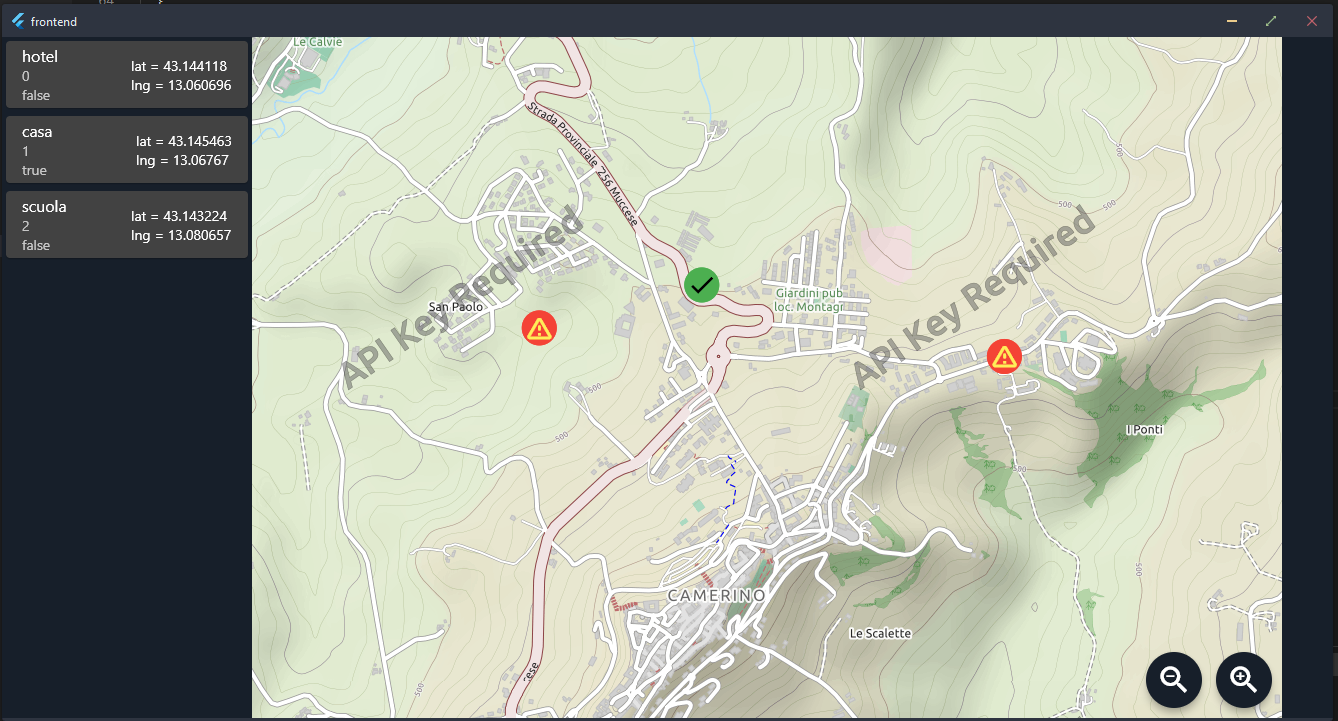
\includegraphics[width=\textwidth]{figure/marker_flutter.png}
    \caption{Marker Flutter}
    \label{marker_flutter}
\end{figure}

Per quanto riguarda il funzionamento offline della mappa l'eseguibile prende in input latitudine e longitudine di un punto e genera un file \textit{tiles.zip} contenente la directory
\setnewpathsep{/} \directory{./tiles/\{z\}/\{x\}/\{y\}/*.png} che va da zoom 15 (scala 1:15 mila) a zoom 22 (scala 1:15 mila) 


L'unico requisito che non è stato soddisfatto a pieno è stato quello di disegnare la heatmap, in quanto necessitavamo di visualizzare una mappa di calore che, in base alla scala della mappa, si ridisegnasse mettendo in relazione la distanza dei punti e l'RSSI rilevato (\textit{Received Signal Strength Indication}).

Come si può notare nella Figura~\ref{heatmap_flutter}, abbiamo disegnato dei punti che tenevano conto dell'RSSI ma non siamo stati in grado di tenere in considerazione la densità dei punti. Questo ci portava a visualizzare una heatmap che, se avevamo tanti punti vicino ma tutti con intensità molto bassa venivano disegnati di verde, invece noi necessitavamo che in questa circostanza la zona interessata fosse colorata di rosso. 
\begin{figure}[tbp]
    \centering
    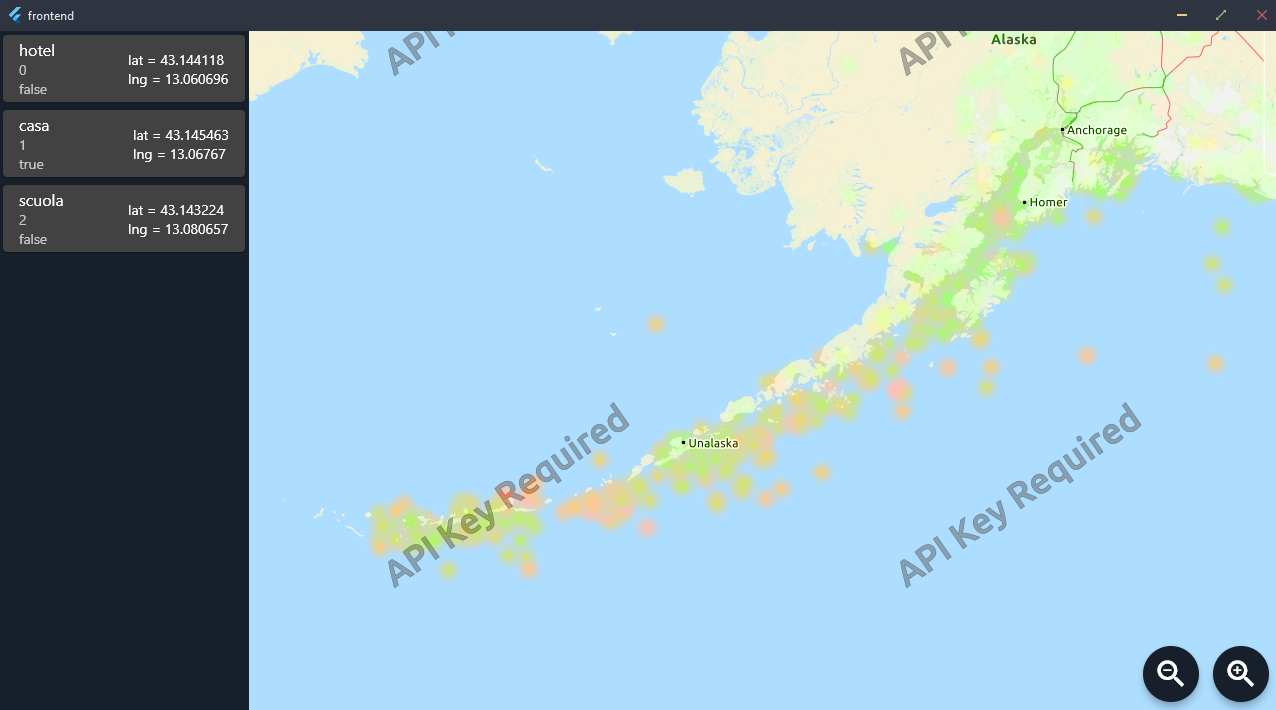
\includegraphics[width=\textwidth]{figure/heatmap_flutter.png}
    \caption{Heatmap Flutter}
    \label{heatmap_flutter}
\end{figure}

\addcontentsline{toc}{section}{Riferimenti bibliografici}
\printbibliography

\end{document}